\documentclass{article}

\usepackage{amsmath}
\usepackage{amssymb}
\usepackage{cleveref}
\usepackage{fullpage}
\usepackage{graphicx}

\begin{document}

\section*{Idea: just-in-time local penumbra in 3D}

\paragraph{Basic idea.} Qi and Vladimirsky developed a method for
local factoring in 2D, as well as an algorithm based on geometric
considerations that allows for just-in-time local factoring which
identifies point sources associated with rarefaction fans. They define
\emph{regular obstacles (for a given point source)} as ones which have
some characteristics emanating from a point source leading into the
obstacle, and \emph{rarefying obstacles} as ones that don't. In their
paper, they don't delve too deeply into the details, but in 2D, this
situation is summarized by \cref{fig:2d-factoring}, which shows a
rarefying obstacle.

\paragraph{Cone + plane factoring.} In Qi and Vladimirsky's Algorithm
2, it appears that when doing local factoring, they ``factor'' all
points that are within a distance $r$ of a point source (corresponding
to a rarefaction fan or otherwise). For a point source that generates
a rarefaction fan, points that don't lie in the rarefaction fan are
also factored. They claim that if the $T(x) = s(x_0) \|x - x_0\|$
(where $x_0$ is the point source) definition is used in this case, it
doesn't provide the proper order of convergence. To compensate for
this effect, they introduce a $T(x)$ function which sets $T$ to be
linear outside of the rarefaction fan (see their paper for a
plot). \emph{It's unclear if this is even necessary}---it seems
intuitive that by \emph{only} factoring points that lie in the
rarefaction fan, the default $T(x) = s(x_0)\|x - x_0\|$ definition can
be used, but this requires identifying which points lie in the
rarefaction fan. This should be doable, though, since it's a
straightforward geometry problem (again, see
\cref{fig:2d-factoring}). It's not clear to me whether they considered
this idea in their paper.

\paragraph{Local factoring in 3D.} The situation in 3D is
significantly more complicated. For a point source which scatters and
diffracts around, e.g., a convex polyhedron, there are potentially
many shadow zones corresponding to rarefaction fans which need to be
identified, each of which can be defined as a polyhedral/pyramidal
(affine) cone or wedge. See \cref{fig:3d-factoring,fig:zone-types}.

A further complication lies in the fact that unlike in the 2D case,
the shadow zones will typically expand from lines of points (line
sources) instead of just single points. We can call these zones
\emph{penumbra}. This means that we require a new definition for
$T$. If we let $E$ be an edge or line of points which constitute the
origin of a rarefaction fan (for example, either the top rim or bottom
rim of the box in \cref{fig:2d-factoring,fig:3d-factoring}), then:
\begin{equation}
  T(x) = \min_{x_0 \in E} s(x_0) \|x - x_0\|,
\end{equation}
where $T$ is defined on a penumbra $P$. If $s \equiv 1$, then defining
$T$ is a little complicated but not impossible (a geometry problem
which may be a little tricky to program), but it seems unlikely that
this function will have a closed form solution for arbitrary $s$, in
which case we will need to design a procedure to compute it for each
$P$ in the domain (after locating and building each $P$!).

One more problem: imagine that we have an obstacle with many, small
facets (e.g.\ a triangle mesh). If the factoring radius $r^\circ$ is
too large, then factored regions could easily bump into other regions.

\paragraph{Diffraction in high-frequency acoustics.} If we can come up
with a way to compute the amplitude in each penumbra using some theory
which describes how amplitude diminishes as sound diffracts around a
corner or a wedge, we can then extend the Popov algorithm to compute
the high frequency approximation to the Helmholtz equation throughout
the domain. A benefit of this approach is that we get---as a bonus---a
significantly more accurate eikonal $\tau$, which can only improve the
accuracy of $\alpha$ and the overall wave field $W$.

\begin{figure}[t]
  \centering
  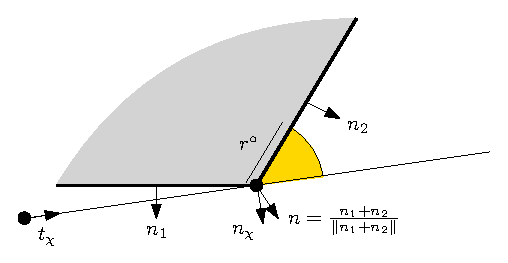
\includegraphics{2d-factoring.eps}
  \caption{The local factoring setup in 2D. A ray strikes the corner
    of the obstacle (gray region) at an oblique angle, creating a
    rarefaction in its shadow (yellow region). The letter $\chi$
    denotes the ray ($\chi$ for \emph{ch}aracteristic): $t_\chi$ and
    $n_\chi$ are its normal and tangent vectors. The normal $n_\chi$
    is chosen so that $\langle t_\chi, n_\chi \rangle = 0$ and
    $\langle n_\chi, n \rangle \geq 0$. The shadow zone is the
    intersection of unoccluded space and the cone spanned by $t_\chi$
    and $-n_\chi$. In this case, the relevant unoccluded space is
    defined by the affine halfspace corresponding to
    $n_2$.}\label{fig:2d-factoring}
\end{figure}

\begin{figure}[t]
  \centering
  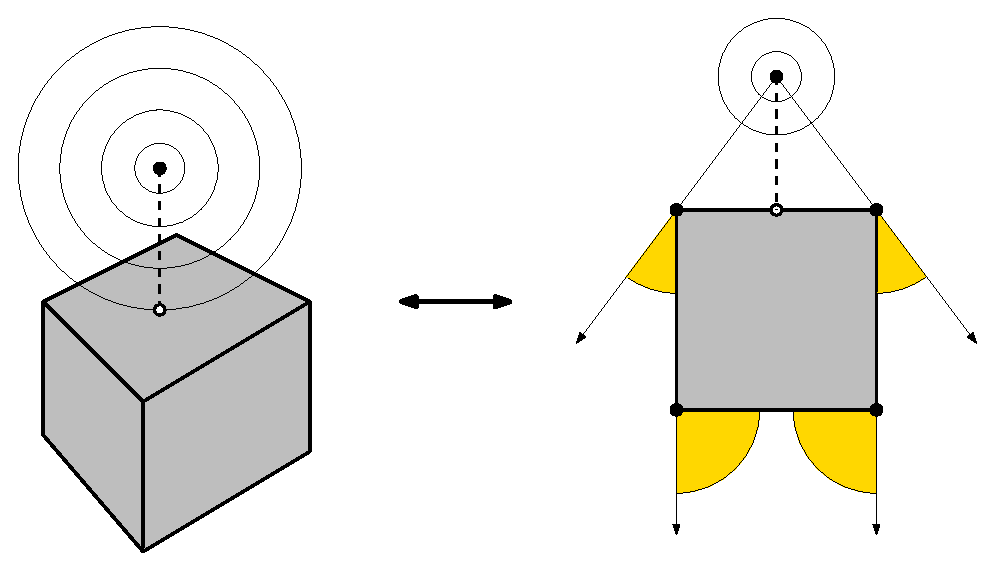
\includegraphics[width=0.8\linewidth]{3d-factoring.eps}
  \caption{Local factoring in 3D. A point source which hovers above a
    box-shaped obstacle emits and creates lines of rarefaction fans
    along its edges. Left: the general 3D setup---the dotted line
    ending in a filled white circle is the minimum distance projection
    of the point source onto the box, to give some sense of
    orientation. Right: a slice in the $yz$-plane showing how lines of
    rarefied point sources are created. Compared with the simpler
    setup in 2D, points in the wedge-shaped shadow that lines the top
    edge of the box like a gutter will need to be simultaneously
    factored using a more complicated $T$ function. We can call these
    combined shadow regions \emph{penumbra}.}\label{fig:3d-factoring}
\end{figure}

\begin{figure}[t]
  \centering
  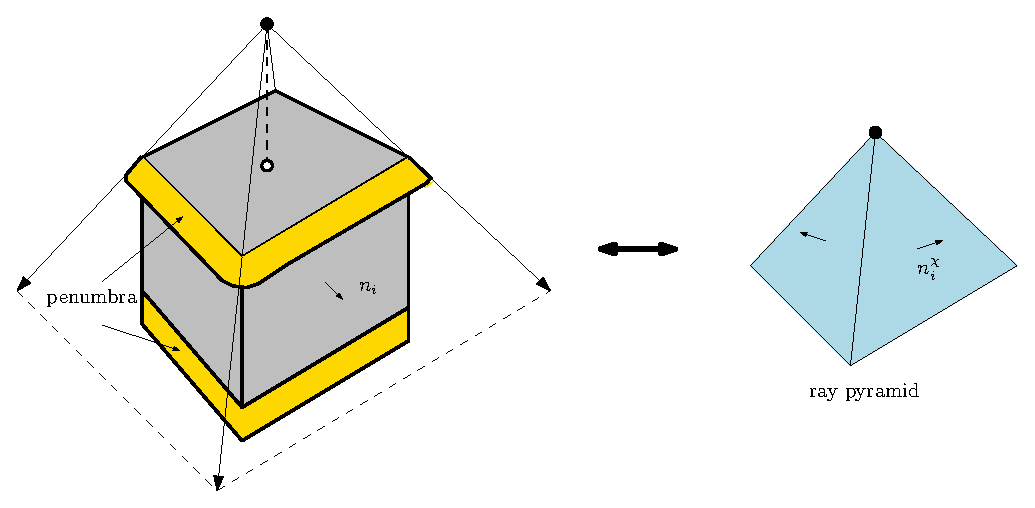
\includegraphics[width=0.9\linewidth]{zone-types.eps}
  \caption{Left: a 3D view of the two penumbra created by a point
    source diffracting around a box obstacle. Right: the rays that
    strike the nearest face of the box span a pyramidal cone with four
    sides. We can define facets for this cone which have normals
    $n_i^\chi$ which will play the role of the ray normal $n_\chi$ in
    \cref{fig:2d-factoring}. Likewise, we define box side normals
    $n_i$, which are analogous to $n_1$ and $n_2$ in
    \cref{fig:2d-factoring}. We number the pyramid normals $n_i^\chi$
    and $n_i$ so that they are matched. Let $H(n)$ be the affine
    halfspace associated with a given normal in the preceding
    setup. As an example, one way to construct the top of the two
    penumbra would be to intersect the halfspaces associated with each
    $n_i$ and $n^\chi_i$ to get $H(n_i) \cap H(n^\chi_i)$, take their
    union to get $Z = \bigcup_i (H(n_i) \cap H(n^\chi_i))$, and then
    consider the set of points
    $P = \{p \in Z : p \mbox{ is within a distance of } r^\circ \mbox{
      from a point on the top edge of the
      box}\}$.}\label{fig:zone-types}
\end{figure}

\begin{figure}
  \centering
  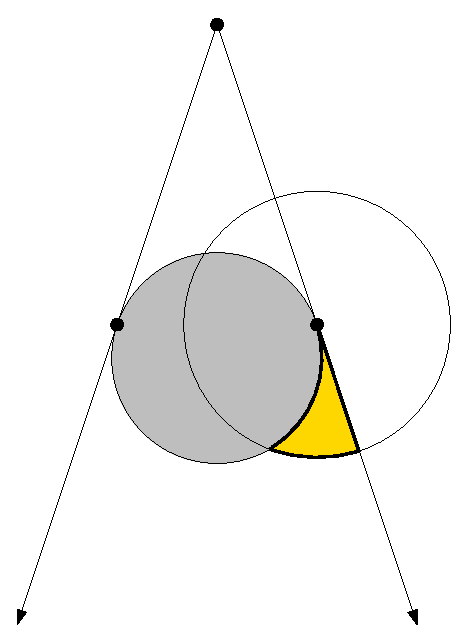
\includegraphics{circle-diffract.eps}
  \caption{tmp}
\end{figure}

\end{document}

%%% Local Variables:
%%% mode: latex
%%% TeX-master: t
%%% End:
